%\documentclass[3p,preprint]{elsarticle}
\documentclass[3p,twocolumn]{elsarticle}
\usepackage[colorlinks,citecolor=blue]{hyperref}
\usepackage{lineno}
\usepackage{amsmath}
\usepackage{ifthen}
\usepackage{commath}
\usepackage{amssymb}
\usepackage{scalerel}
\usepackage{natbib}
\usepackage[version=4]{mhchem}

\usepackage{adjustbox}   
\usepackage{threeparttable}
\usepackage{booktabs}
\usepackage{colortbl} 
\usepackage{xcolor}
\usepackage{mhchem}

\newcommand{\diff}[2]{\dfrac{\partial #1}{\partial #2}}

\usepackage{amsmath}
\usepackage{commath}
\usepackage{graphicx,bm}
\usepackage{epstopdf}
\usepackage{float}
\biboptions{sort&compress}
\modulolinenumbers[5]
\usepackage{subfig}

\usepackage[T1]{fontenc}
\usepackage{xr}
\externaldocument{supp_material}

\journal{Journal of \LaTeX\ Templates}

%%%%%%%%%%%%%%%%%%%%%%%
%% Elsevier bibliography styles
%%%%%%%%%%%%%%%%%%%%%%%
%% To change the style, put a % in front of the second line of the current style and
%% remove the % from the second line of the style you would like to use.
%%%%%%%%%%%%%%%%%%%%%%%
%% Numbered
%\bibliographystyle{model1-num-names}

%% Numbered without titles
%\bibliographystyle{model1a-num-names}

%% Harvard
%\bibliographystyle{model2-names.bst}\biboptions{authoryear}

%% Vancouver numbered
%\usepackage{numcompress}\bibliographystyle{model3-num-names}

%% Vancouver name/year
%\usepackage{numcompress}\bibliographystyle{model4-names}\biboptions{authoryear}

%% APA style
%\bibliographystyle{model5-names}\biboptions{authoryear}

%% AMA style
%\usepackage{numcompress}\bibliographystyle{model6-num-names}

%% `Elsevier LaTeX' style
\bibliographystyle{elsarticle-num}
%%%%%%%%%%%%%%%%%%%%%%%

\begin{document}

\begin{frontmatter}

\title{A molecular dynamics study of the solvation of \ce{CO_2}, water, and some organic compounds in the ionic liquids \ce{[emim][B(CN)_4]} and \ce{[emim][NTf_2]}}

%% Group authors per affiliation:
\author[rvt]{A.J.~Silveira}
\author[rvt]{S.~Pereda}
\author[focal,els]{F.W.~Tavares}
\author[focal]{C.R.A.~Abreu\corref{cor1}}
\ead{abreu@eq.ufrj.br}

\address[rvt]{Planta Piloto de Ingenier\'ia Qu\'imica, PLAPIQUI, Universidad Nacional del Sur,Camino La Carrindanga Km 7-CC: 717, Bah\'ia Blanca, Argentina}
\address[focal]{Chemical Engineering Department, Escola de Qu\'imica, Universidade Federal do Rio de Janeiro,Rio de Janeiro, RJ 21941-909, Brazil}
\address[els]{COPPE, Universidade Federal do Rio de Janeiro, Rio de Janeiro, RJ 21941-909, Brazil}

\cortext[cor1]{Corresponding author}

\begin{abstract}
In this paper, we calculate solvation free energies in ionic liquids and predict macroscopic properties required in the design of chemical processes.
Carbon dioxide from combustion processes is one of the main sources of anthropogenic generation of greenhouse gases.
On the other hand, the potential of \ce{[emim][B(CN)_4]} for its capture has recently been reported.
For comparison, the solvents \ce{[emim][B(CN)_4]} and \ce{[emim][NTf_2]} are analyzed, both at infinite dilution and at high concentrations of \ce{CO_2}.
Our results confirm what is experimentally observed, namely a considerably lower pressure is required to dissolve a certain amount of \ce{CO_2} in \ce{[emim][B(CN)_4]}.
The infinite-dilution activity coefficients of hexane, benzene, cyclohexane, ethanol, and water in \ce{[emim][B(CN)_4]} are also calculated, and a comparison is made with experimental values recently reported in literature.
\end{abstract}

\begin{keyword}
ionic liquids \sep solvation free energy \sep  \ce{CO_2} Henry constant \sep infinite-dilution activity coefficient 
\end{keyword}

\end{frontmatter}

\linenumbers

\section{Introduction}
\ce{CO_2} emissions from fossil-fuel power generation plants account for a large portion of the anthropogenic greenhouse gases \cite{totalenergy}.
International efforts aimed at regulating and reducing \ce{CO_2} emissions are increasing \cite{Tong_2018} and, in this context, the development of technologies for the capture and storage of \ce{CO_2} plays an essential role \cite{Markewitz_2014}. 

The conventional process for \ce{CO_2} removal comprises a chemical absorption followed by stripping at high temperatures.
The most commonly used solvents are volatile organic compounds, specially aqueous solutions of monoethanolamine (MEA).
Despite its high absorption capability, the use of MEA suffers from a serious drawback due to the high cost of solvent recovery \cite{Merkel_2010}.
Other disadvantages include corrosion and degradation by oxidation, solvent loss by evaporation, which also contributes to increase the environmental pollution and generates extra costs for replacing the solvent.

The use of ionic liquids (ILs) as solvents for \ce{CO_2} sequestration occupies a central place in the investigation of alternative technologies.
The reasons are their well known properties, such as their almost negligible vapor pressure and high thermal stability.
Furthermore, they are particularly attractive since they can be designed for specific applications, giving rise to the so-called task-specific ILs \cite{Seo_2014}.
These remarkable properties makes ILs suitable for a wide variety of applications in separation processes \cite{Han_2010,Werner_2010}, catalysis \cite{P_rvulescu_2007}, energy \cite{MacFarlane_2014}, and material science \cite{Mecerreyes_2011,Tom_2015,Dupont_2010,Leones_2017,Kinik_2017}.

Recently, the potentiality of ILs for \ce{CO_2} capture has been called into question by Carvalho \textit{et al.} \cite{Carvalho_2016}, who warn that the use of molar fraction to express solubility has, to some extent, perpetuated misconceptions regarding the supposed absorption capability of certain ILs.
Although most thermodynamic models are formulated in terms of molar fraction, a key factor that dictates the absorption process efficiency is given by the amount of \ce{CO_2} that can be dissolved in a certain \textit{volume} or \textit{mass} of solvent.
By expressing the solubility values in terms of molality and performing an exhaustive comparison between various ILs, Ref. \cite{Carvalho_2016} shows that most systems which promote a physical absorption of \ce{CO_2} exhibit a solubility similar, or even lower, than that observed for the heavy alkane eicosane.
This is true for the ``popular'' \ce{[bmim][NTf_2]}, \ce{[bmim][PF_6]}, \ce{[bmim][BF_4]}, as well as for those synthesized from the fluorination of the cation or the anion, such as \ce{[(C_2H_2F_2)mim][NTf_2]} and \ce{[hmim][pFAP]}; the only exception being the family of ILs containing the anion tetracyanoborate \ce{[B(CN)_4]^-}.

There is no obvious explanation accounting for the enhanced solubility promoted by the presence of \ce{[B(CN)_4]^-}.
In this context, molecular simulation provides with a powerful tool for studying solvation processes.
To the best of our knowledge, only one study in literature reports the free energy of solvation of \ce{CO_2} in \ce{[emim][B(CN)_4]} \cite{Liu_2014_1} which, in addition, is overestimated.
This motivated us to evaluate different force fields of \ce{[emim][B(CN)_4]} and, as we will show below, it was possible to find a model that successfully reproduces the experimental value of the Henry constant of \ce{CO_2}.
For comparison, \ce{[emim][B(CN)_4]} and \ce{[emim][NTf_2]} were analyzed, both at infinite dilution and at high concentrations of \ce{CO_2}.
The simulations confirmed what is observed in experiments: for \ce{[emim][B(CN)_4]}, a considerably lower pressure is required to dissolve the same amount of \ce{CO_2}.
The infinite-dilution activity coefficients of solutes hexane, benzene, cyclohexane, ethanol, and water in \ce{[emim][B(CN)_4]} were also calculated, and a comparison was made with experimental values recently reported in literature.

This paper is organized as follows: in Sec.~\ref{sec:theory} we present the theoretical background, which is followed by a brief description of the force fields used in this work.
The methodological details are provided in Sec.~\ref{sec:sim_details} and the corresponding numerical results are given in Sec.~\ref{sec:results}.
Finally, we present some concluding remarks in Sec.~\ref{sec:conclusion}.

\section{Theoretical background}
\label{sec:theory}

In this section, we present the formalism that allows us to compute the Henry constant and activity coefficient, both at infinite dilution, from the simulated free energy.
For this, we rely on the work of Shirts \textit{et al.} \cite{Shirts_2003}.
Then, we reformulate the equations in order to study concentrated solutions, which would be the more likely scenario in \ce{CO_2} capture processes.

\subsection*{Solvation free energy}
The solvation free energy, $\Delta G_{\text{solv}}$, is defined as the reversible work needed to transfer a solute molecule from the gas phase to the solution.
For dense systems, an efficient computation of solvation properties via molecular simulation is possible by means of the so-called alchemical methods, which employ non-physical pathways to connect the ``endpoint'' states, whose free energy difference is to be estimated.
In the case of $\Delta G_{\text{solv}}$, the alchemical route involves a gradual insertion/deletion of the solute through the use of a coupling parameter $\lambda$, which scales the intermolecular interactions taking values in the interval [0,1]: $\lambda$ = 1 corresponds to a fully interacting system, while for $\lambda$ = 0 the interactions between the solute and solvent molecules are completely turned-off.

In the following, the subscripts ``$s$'' and ``$\text{IL}$'' refer to the solute and the solvent (ionic liquid), respectively.
For a system containing $N_{\text{IL}}$ solvent molecules and $N_{\text{s}}$ solute molecules at fixed pressure (P) and temperature (T), the difference in free energy between the states associated to $\lambda$ = 1 and $\lambda$ = 0 is formally defined as
\begin{equation}
\Delta G_{\text{sim}} \equiv k_b T \ln \frac{\bigtriangleup (N_s^l,N_{\text{IL}},P,T,\lambda = 1)}{\bigtriangleup (N_s^l,N_{\text{IL}},P,T,\lambda = 0)}, 
\end{equation}
where superscript ``$l$'' refers to the liquid solution, $\bigtriangleup$ denotes the isobaric-isothermal partition function, and $k_b$ is the Boltzmann's constant.
Shirts \textit{et al.} \cite{Shirts_2003} rigorously derived the working expression that relates $\Delta G_{\text{sim}}$ to what is experimentally known as the solvation free energy.
They found out that
\begin{equation}
\begin{split}
\label{eq:free_solv}
 \Delta G_{\text{solv}}& =  k_b T \ln \left( \frac{P_s}{c_s^{\ast} k_b T} \right)\\ &= \Delta G_{\text{sim}} - k_bT \ln \left( \frac{V^{\ast}}{V_1} \right),
\end{split}
\end{equation}
where $V^{\ast}$ and $V_1$ refer to the mean volumes of the systems specified by ($N_s^l-1$,$N_{\text{LI}}$,P,T) and ($N_s^l$,$N_{\text{LI}}$,P,T), respectively; $c_s^{\ast}$ = $N_s^l/V_1$ is the numerical concentration of the solute in the liquid-phase and $P_s$ is the partial pressure of the solute in the gas phase.
It should be noted that in the derivation of Eq.~\eqref{eq:free_solv}, the gas phase is treated as an ideal gas. 

For small solutes, such as those considered in this work, the magnitude of the term $V^{\ast}/V_1$ is typically on the order of the free energy uncertainties \cite{Shirts_2003}.
Hence, that term can be neglected and will be omitted hereafter.

\subsection*{Henry constant}
If both $P_s$ and $c_s^{\ast}$ were not large, we can resort to Eq.~\eqref{eq:free_solv} to predict Henry's law constant $\text{K}_s$, which is defined as \cite{Prausnitz}
\begin{equation}
\text{K}_s =\frac{P_s}{x_s}.
\end{equation}
Therefore, by simply expressing Eq.~\eqref{eq:free_solv} in terms of the molar fraction $x_s$ and assuming that MW (molecular weight of the solution) = $\text{MW}_{\scaleto{IL}{4pt}}$, as well as $\rho$ (mass density of the solution) = $\rho_{\scaleto{IL}{4pt}}$, we obtain that
\begin{equation}
\label{eq:henry_eq}
K_s = \tilde{\rho}_{\scaleto{IL}{4pt}} R \, T \exp(\beta \, \Delta G_{\text{sim}}),
\end{equation}
where $\tilde{\rho}_{\scaleto{IL}{4pt}}$ is the molar density of the solvent and $R$ is the gas constant.

\subsection*{Partial pressure estimation}
\label{sec:partial_pressure}

For the ILs of interest to the present investigation, high concentrations of \ce{CO_2} are found at pressure values for which, in principle, the ideal gas assumption may be not valid.
In this case, we shall correct the ideal gas contribution to the chemical potential, as follows
\begin{equation}
\label{eq:mu_gas_real}
\mu^{g}_s = \mu^{ig}_s + RT \ln \phi_s,
\end{equation}
where $\phi_s$ is the fugacity coefficient of the solute.
This equation, together with the fact that $f^{g}_s$ = $P_s \phi_s$, are used to evaluate $\mu^{l}_s$ = $\mu^{g}_s$, which yields
\begin{equation}
\label{eq:fgas_d}
f^{g}_s = \exp  \left( \beta \Delta G_{\text{sim}} \right) +  k_b T c_s^{\ast}, 
\end{equation}
where $f^{g}_s$ is the fugacity of the solute in the gas phase.
Having calculated $f^{g}_s$, $P_s$ can be predicted using the following equation
\begin{equation}
\label{eq:fgas}
f^{g}_s = P_s \exp\left[ \frac{B_s(T) P_s}{R T} \right],
\end{equation}
where $B_s$ corresponds to the second virial coefficient.
Here, we employ the correlation of $B_s$ for \ce{CO_2} introduced by Holste \textit{et al.} \cite{Holste_1987}, which is
\begin{equation}
B_s = B_0 + \frac{B_1}{T} + \frac{B_2}{T^2},
\end{equation}
where $B_0$ = 23.02991 cm$^3$/mol, $B_1$ = -2.455297 $\times$ 10$^3$ (Kcm$^3$/mol) and $B_2$ = -1.22675$\times$10$^7$ (K$^2$cm$^3$/mol).

As supported by preliminary simulations, it seems reasonable to assume $\Delta G_{\text{sim}}$ as independent of pressure over the range of experimental data considered in this work.
Then, the equilibrium pressure is determined by directly solving Eq.~\eqref{eq:fgas} for $P_s$.

\subsection*{Infinite-dilution activity coefficient}

As will be shown below, the prediction of activity coefficients requires extra simulations involving the pure solute.
In what follows, we use the superscript ``$0$'' to denote the pure solute properties.

Using standard thermodynamic relations \cite{Tester}, we write the activity coefficient $\gamma_s$ in terms of residual chemical potentials, as follows:
\begin{equation}
\label{eq:gamma}
\ln \gamma_s = \frac{1}{RT} (\mu_s^R - \mu_s^{R,0}),
\end{equation}
where $\mu_s^R$ and $\mu_s^{R,0}$ are the residual chemical potentials of the solute in the solution and in the pure solute, respectively.
It is worth noting that we have used the definition $\mu_s^{R}$ (P,T) = $\mu_s$ (P,T) - $\mu_s^{ig}$ (P,T), where the superscript $ig$ refers to a solution of ideal gases.
Also, recall that $\mu_s^{ig} (P,T)$ = $\mu_s^{ig,0} (P,T)$ + $RT \ln x_s$, so we have that
\begin{equation}
\mu_s^R = \mu_s^l(N_s^l,N_{LI},P,T) - \mu_s^{ig,0}(P,T) - k_b T \ln x_s.
\end{equation}
Replacing $\mu_s^{l}$ and $\mu_s^{ig,0}$ by the corresponding expressions derived in Ref.~\cite{Shirts_2003} yields
\begin{equation}
\label{eq:mu_res}
\mu_s^R = \Delta G_{\text{sim}} - k_b T \ln \left( \frac{V^{\ast} P}{N_s^l k_b T} \right) -  k_b T \ln x_s.
\end{equation}
Of course, an analogous equation holds for $\mu_s^{R,0}$:
\begin{equation}
\label{eq:mu_res_0}
\mu_s^{R,0} = \Delta G_{\text{sim}}^{0} - k_b T \ln \left( \frac{V^{\ast,0} P}{N_s^{l,0} k_b T} \right).
\end{equation}

If one makes $N_s^{l}$ = 1, and substitute Eqs.~\eqref{eq:mu_res} and~\eqref{eq:mu_res_0} into Eq.~\eqref{eq:gamma}, the infinite-dilution activity coefficient, $\gamma^{\infty}_s$, can be predicted according to the following equation:
\begin{equation}
\label{eq:gamma_inf}
\ln \gamma^{\infty}_s = \frac{1}{k_b T} \left( \Delta G_{\text{sim}} - \Delta G_{\text{sim}}^{0} \right) + \frac{c_{\scaleto{LI}{4pt}}^{\, \ast}}{c_{\, s}^{\, \ast,0}},
\end{equation}
where $c_{\scaleto{IL}{4pt}}^{\, \ast}$ y $c_{\, s}^{\, \ast,0}$ are the numerical densities of the solvent and the pure solute, respectively.

\section{Force fields}
\label{sec:force_field}
\subsection{Ionic liquids}
\label{sec:force_field_il}

The versatility of ILs for different applications is in part due to the fact that their physical properties strongly depend on the particular cation-anion combination.
On the other hand, this feature also explains why the desirable transferability of force fields is particularly difficult to attain.
Indeed, it is a common practice to extract the potential parameters of the intramolecular (bond stretching, angle bending, torsion rotation) and Lennard-Jones (LJ) interactions from a well established force field and, then, only derive the partial atomic charges with the aim of ``adjusting'' the model for a specific pair of ions.
This procedure is, however, inaccurate as in conventional force fields the determination of the atomic charges precedes the dihedrals parametrization.
Another ad-hoc strategy, which intends to crudely incorporate polarization effects, is to scale the partial charges uniformly with a factor which normally takes values in the range 0.8-0.9.
This has proven to be effective for predicting dynamic properties \cite{Schr_der_2012}.

In this paper, we consider four models of \ce{[emim][B(CN)_4]}.
Koller \textit{et al.} \cite{Koller_2012} were the first to introduce a specific non-polarizable force field for that IL.
They tested three variations of a \textit{united-atoms} model, in which the alkyl groups \ce{CH_3} and \ce{CH_2} of \ce{[emim]^+} are replaced by pseudo-atoms.
Among them, the ``FF-3'' model best reproduces the experimental values of density, self-diffusion coefficients and viscosity.
In short, both the intramolecular and LJ parameters of the cation were taken from the work of Liu \textit{et al.} \cite{Liu_2006}, which in turn is based on the AMBER \cite{Cornell_1995} framework.
The intramolecular parameters involving the boron atom were extracted from the DREIDING \cite{Mayo_1990} force field and the anionic vdW parameters were refined based on the values reported by Price \textit{et al.} \cite{Price_2001}.
The atomic partial charges were derived using the EA-RESP method \cite{Basma_2001} from \textit{Post-Hartree-Fock ab-initio} calculations at MP2/6-31G$^\ast$+ level of theory, which automatically resulted in total charges on the ions of $\pm$0.8426$e$. 

The potential parameters of \ce{[B(CN)_4]^-} derived by Koller \textit{et al.} \cite{Koller_2012} were then used by Batista \textit{et al.} \cite{Batista_2015} to study aqueous solutions of \ce{[emim][B(CN)_4]}.
In this case, the authors considered the \textit{all-atom} model of \ce{[emim]^+} developed by Cadena and Maginn \cite{Cadena_2006}.
The atomic partial charges were obtained using the CHELP procedure \cite{Breneman_1990}, resulting in net charges of $\pm$0.889$e$ on the ions.
It should be noted that the factors for scaling the 1-4 non-bonded interactions are different for these force fields: Cadena and Maginn \cite{Cadena_2006} apply factors of 1.0 and 0.4 for the LJ and Coulombic interactions, respectively; while in Koller \textit{et al.} \cite{Koller_2012} the corresponding values are 0.5 and 5/6, in accordance with the AMBER force field.
Batista \textit{et al.} \cite{Batista_2015} used the first ones (J.P. Coutinho, personal communication).

Another set of parameters for \ce{[emim][B(CN)_4]} was derived by Liu \textit{et al.} \cite{Liu_2014} in a study that investigates the dynamics of \ce{CO_2} and \ce{N_2} in that IL.
Parameters corresponding to the intramolecular and LJ interactions were extracted from GAFF \cite{Wang_2004}, while the atomic partial charges were computed using the RESP method \cite{Bayly_1993} from \textit{DFT}/B3LYP/6-311+G(d) calculations.
The net charges of the ions were manually adjusted to a value of $\pm$0.8$e$.

We also consider the parametrization reported by Weber and Kirchner \cite{Weber_2016}, which is based on the force field developed by P{\'{a}}dua and Canongia Lopes~\cite{Canongia_Lopes_2006}.
The potential parameters for the anion are not specified in Refs.~\citenum{Weber_2016} and~\citenum{Canongia_Lopes_2006}, and we obtained them by a direct communication with the authors of Ref.~\citenum{Weber_2016}.
The atomic partial charges were derived using the RESP procedure from \textit{Hartree-Fock} calculations at 6-31++G$^{\ast \ast}$ level of theory, resulting in net charges of $\pm$0.8$e$.

Finally, for \ce{[emim][NTf_2]} we use the model of K\"{o}ddermann~\textit{et al.} \cite{K_ddermann_2007}, which was derived by refining the force field due to P{\'{a}}dua and Canongia Lopes \cite{Canongia_Lopes_2006}.
This refining was characterized by their authors as ``unusual'', given that the LJ parameters were modified, while keeping the partial charges at their original values.
This model was recently employed by Kerl \textit{et al.} \cite{Kerl__2017}, who were able to accurately predict Henry constants of \ce{CO_2} at several temperatures.

\subsection{Solutes}
\label{sec:force_field_sol}

The solutes considered in this work are hexane, benzene, \ce{CO_2}, ethanol, cyclohexane and water.
Hexane and benzene were modeled using the OPLS-AA force field \cite{Jorgensen_1996}, while the TRAPPE potential \cite{Chen_2001,Potoff_2001} was employed for ethanol and \ce{CO_2}.
Cyclohexane was simulated using a rigid-body model \cite{munoz2015lennard} whose sites only interact via a LJ potential
For water, we employ the TIP4P/2005 model \cite{Abascal_2005,Vega_2011}. 

\section{Computational methods}
\label{sec:sim_details}

With the aim of setting up a computationally efficient protocol for the ILs, in this work we assess the possibility of modeling the ions as rigid bodies and employing the damped shifted force (DSF) method \cite{Fennell2006} for computing the electrostatic interactions.
As an alternative to the Ewald schemes \cite{Ewald_1921,Darden_1993,Hockney_1988}, McCann \textit{et al.} \cite{McCann_2013} tested the DSF method for various ILs modeled with the OPLS-AA force fields.
They concluded that using $\alpha$ = 0.2 {\AA}$^{-1}$ and a cutoff distance ($r_c$) of 15 {\AA} provide the best energetic agreement with the Ewald method.
In this work, comparisons are made in terms of the simulated densities and radial distribution functions for which, as will be shown in the next section, $\alpha$ = 0.2 {\AA}$^{-1}$ and $r_c$ = 12 {\AA} resulted in a good agreement.
These values were also employed for the charged solutes, with the exception of hexane, for which we applied undamped Coulombic interactions improving the prediction of the chemical potential.

The NPT algorithm of Kamberaj \textit{et al.} \cite{Kamberaj_2005} was used to perform the simulations with rigid bodies.
For flexible molecules, we applied the scheme due to Shinoda \textit{et al.} \cite{Shinoda2004} and C-H bonds were constrained by the SHAKE method \cite{Ryckaert1977}.
For both integrators, we used a time-step size ($\Delta t$) of 1 fs.

The gradual insertion/deletion of charged solutes involves scaling both the van der Waals (vdW) and the electrostatic intermolecular interactions.
In order to avoid numerical instabilities associated to the vdW scaling, a standard approach is to employ a soft-core potential with a nonlinear coupling.
In this paper we use the modified LJ potential due to Beutler \textit{et al.} \cite{Beutler_1994}.
The electrostatic interactions, on the other hand, can be handled by a linear scaling \cite{Naden_2015}.
Furthermore, the contributions to $\Delta G$ originating at the different couplings are taken into account separately, as follows:
\begin{equation}
\begin{split}
\Delta G_{\text{sim}} =& \; \Delta G_{\,\text{vdW}} (\lambda_{\,\text{vdW}} = 0\rightarrow  1, \lambda_{\, \text{Coul}} = 0) \\
+ \; &\Delta G_{\,\text{Coul}} (\lambda_{\, \text{vdW}} = 1,\lambda_{\,\text{Coul}} = 0 \rightarrow 1),
\end{split}
\end{equation}
where $\lambda_{\,\text{vdW}}$ and $\lambda_{\,\text{Coul}}$ are the coupling parameters of the soft-core and electrostatic potentials, respectively.
Note that in the process of coupling the vdW interactions, the Coulombic interactions are turned-off, while we set $\lambda_{\,\text{vdW}}$ = 1 when computing $\Delta G_{\,\text{Coul}}$.
This results in the ``end-point'' states given by ($\lambda_{\,\text{vdW}}$=0,$\lambda_{\,\text{Coul}}$=0) and ($\lambda_{\,\text{vdW}}$=1,$\lambda_{\,\text{Coul}}$=1), as expected.
The complete sets of the coupling parameters we use here are $\lambda_{\text{vdW}}$ = $\{0.0$, $0.05$, $0.1$, $0.2$, $0.25$, $0.3$, $0.35$, $0.4$, $0.45$, $0.5$, $0.6$, $0.7$, $0.8$, $0.9$, $1.0\}$ and $\lambda_{\text{Coul}}$ = $\{0.0$, $0.1$, $0.4$, $0.7$, $0.1\}$.

In this work, we carried out independent simulation at each state of $\lambda_{\text{Coul}}$, while the expanded ensemble (EE) method~\cite{Lyubartsev_1992} was applied for sampling the $\lambda_{\,\text{vdW}}$ set.
In short, an EE is constructed as a weighted sum of subensembles, each assuming a different value of the variable chosen to explore the free energy landscape, which in our case is $\lambda_{\,\text{vdW}}$.
This way, the sampling of an EE comprises both sampling each subensamble with fixed variables (N,P,T,$\lambda_{\,\text{vdW}}$) and transitions in $\lambda_{\,\text{vdW}}$.
Thus, a remarkable feature of the EE method is the possibility of exploring the whole alchemical route in a single simulation.
In this work, we perform a sequential sampling of the EE \cite{Chodera_2011_2}, which consists in sampling each subensamble via NPT molecular dynamics (MD) for a determined number of steps $N^{\text{EE}}$ followed by an attempt to change $\lambda_{\,\text{vdW}}$ using MC, and so on.
The $\lambda_{\,\text{vdW}}$ transitions are performed according to an independent sampling scheme \cite{Chodera_2011_2}.
In addition, the set of (arbitrary) weights $\eta$ of the subensambles enters in the acceptance criteria of MC, so it is possible to tune $\eta$ in order to enhance the sampling.
If differences $\eta_i$ - $\eta_j$ were closed to $\Delta G_{ji}$, we expect an uniform sampling in $\lambda_{\,\text{vdW}}$ \cite{Lyubartsev_1992}.
Of course, this can be achieved only iteratively.
The EE procedure, together with the \textit{soft-core} potential and the DSF method with linear coupling were implemented in the LAMMPS software package \cite{Plimpton1995}, which we used for carrying out all the simulations.

As demonstrated in Ref.~\citenum{Chodera_2011_2}, smaller values of $N^{EE}$ yield more decorrelated samples in each subensemble.
In this work, we employed $N^{EE}$ = 5 which, together with the specified $\lambda_{\, \text{vdW}}$ set, required up to 3 preliminary runs of the EE for determining the weights $\eta$ that yielded, in a final simulation, a ``sufficient'' sampling of each subensamble.
By ``sufficient'', we mean that the sampling provides an acceptable uncertainty in $\Delta G$.
The simulation times for the preliminary and final EE runs were 10 and 40 ns, respectively; and each $\lambda_{\text{Coul}}$ state was simulated for 10 ns.
Finally, the MBAR method \cite{Shirts_2008}, as implemented by Klimovich \textit{et al.} \cite{Klimovich_2015}, was applied to estimate $\Delta G_{\text{vdW}}$ and $\Delta G_{\text{Coul}}$.

The initial configurations were obtained with PLAYMOL \cite{playmol}, a software integrated with PACKMOL \cite{Mart_nez_2009}, using the tool \textit{build} to specify geometric data (bond and angle lengths, and dihedral angles), from which PLAYMOL automatically determines the Cartesian coordinates.
We first carried out NVT MD simulations of the isolated ion pairs in order to obtain a minimum energy conformation.
For this, we used the Nos\'{e}-Hoover thermostat \cite{Martyna1992} and a cubic box of length L = 50 {\AA} with non-periodic boundary conditions.
After a short run with $\Delta t$ = $0.5~\text{fs}$, we carried out a ``quenching'' simulation with $\Delta t$ = $1 ~\text{fs}$, in which the temperature is gradually reduced until reaching a value close to $0~\text{K}$.
The resulting coordinates were then specified in PLAYMOL \cite{playmol} to build the configurations of the liquid phases.

\section{Results and discussion}
\label{sec:results}

\subsection{Simulation strategies of ILs}
\label{sec:prel_results}

In this section, we present results for the following two cases: (1) flexible ions together with the Particle-Particle-Particle-Mesh (PPPM) method~\cite{Hockney_1988} with a tolerance of 1$\times$10$^{-4}$ for calculating the Coulombic interactions, and (2) ions modeled as rigid bodies with the DSF method \cite{Fennell2006} ($\alpha$ = 0.2 {\AA}$^{-1}$) as the alternative to the PPPM scheme.
In both cases, $r_c$ = 12 {\AA}.
The nomenclature used in this paper is shown in Fig~\ref{fig:atoms_id}.
In the \textit{united-atoms} version of \ce{[emim]^+}, hydrogens ranging from H4 to H11 are eliminated.

The rigid bodies were built after carrying out an analysis of key dihedrals, whose flexibility could lead to significant conformational changes in \ce{[emim]^+} and \ce{[NTf_2]^-}.
On the other hand, small and highly symmetric anions, such as \ce{PF_6} and \ce{BF_4} are usually modeled as rigid bodies \cite{HANKE_2001,Hanke_2003,Lynden_Bell_2006}, which justifies the strategy in the case of \ce{[B(CN)_4]^-}.

\begin{figure}[ht]
\centering
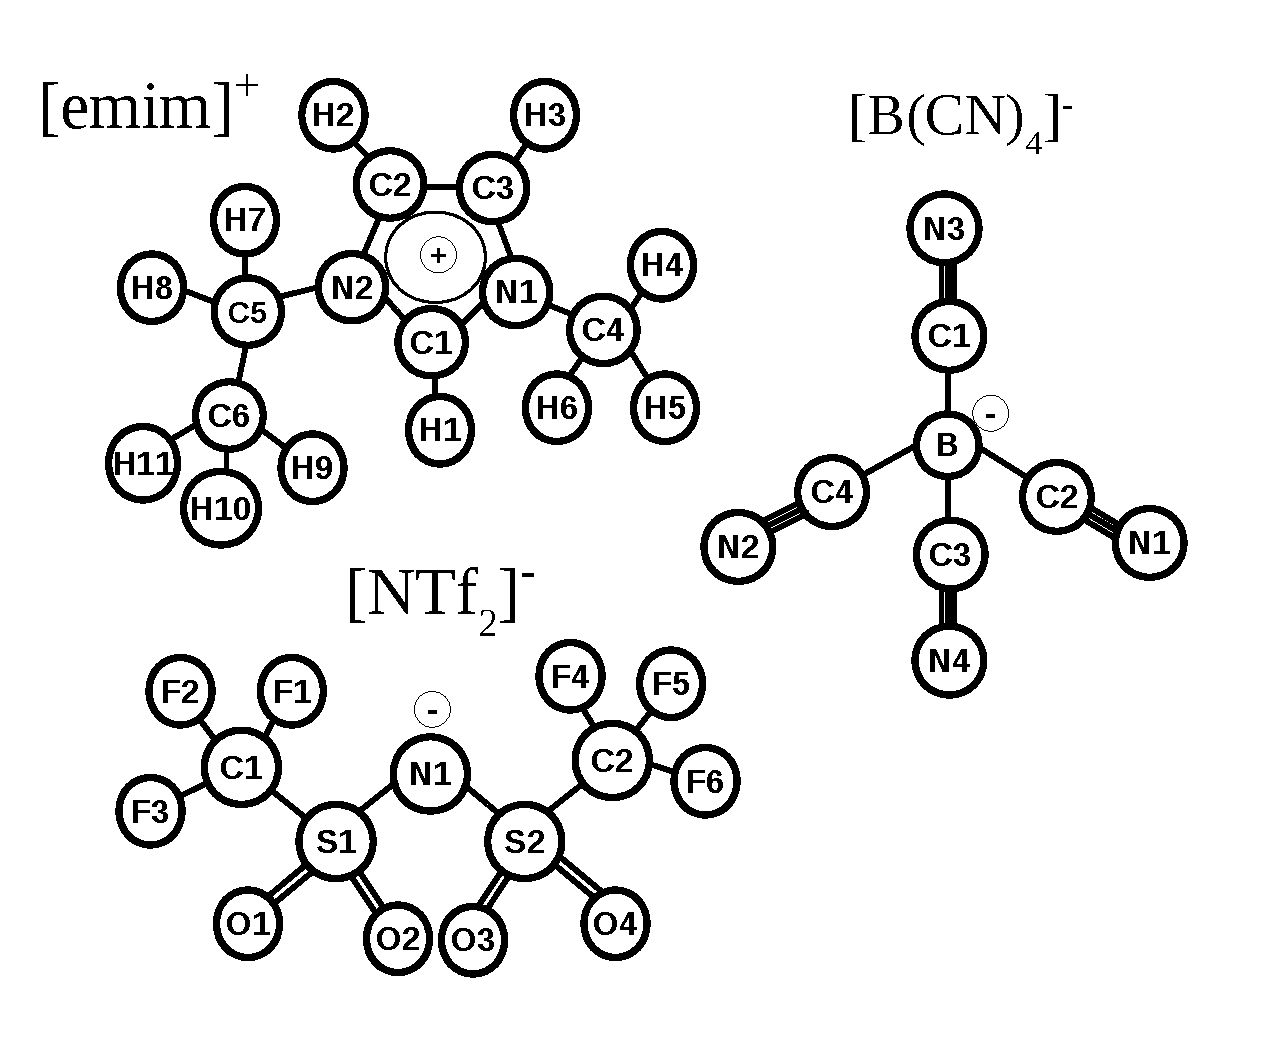
\includegraphics[width=\linewidth]{atoms_id.pdf}
\caption{Adopted nomenclature for 1-ethyl-3-methylimidazolium  (\ce{[emim]^+}), tetracyano borate (\ce{[B(CN)_4]^-}) and bis(trifluoromethylsulfonyl)amide (\ce{[NTf_2]^-}).}
\label{fig:atoms_id}
\end{figure}

Using the software TRAVIS \cite{Brehm_2011}, we obtained the combined distribution functions (CDFs) of the dihedral angles of C1-N2-C5-C6 and C2-N2-C5-C6, as sampled in NPT-MD simulations of 250 ion pairs at $T = 298.0~\text{K}$ and $P = 1.0~\text{bar}$.
In Fig.~\ref{fig:dihedrals_emim} we show the CDFs for each force field of \ce{[emim][B(CN)_4]}.
A first inspection of this figure reveals a similar behavior of the models due to Koller \textit{et al.} \cite{Koller_2012} and Liu \textit{et al.} \cite{Liu_2014}.
This was expected as both are based on the AMBER framework \cite{Cornell_1995}.
In addition, Figs.~\ref{fig:dihedrals_emim}(a) and \ref{fig:dihedrals_emim}(b) are symmetric, which means that atoms C1, N2, and C2 are coplanar.
In Fig.~\ref{fig:dihedrals_emim}(a), the most likely angles can be found in a narrow region around 90$^{\circ}$ and 270$^{\circ}$.
Since these angles correspond to an equivalent configuration in the \textit{united-atom} \ce{[emim]^+}, in the case of Koller \textit{et al.} \cite{Koller_2012} we built all the rigid bodies by specifying 90$^{\circ}$ for the dihedral angle of C6-C5-N2-C1.
The other models show a larger flexibility with high probability regions that extend in a broad range of angle values.
Despite this, it was possible to build more than one type of rigid body by specifying the most probables angles of C6-C5-N2-C1.
In the case of Liu \textit{et al.} \cite{Liu_2014}, these angles correspond to 90$^{\circ}$ and -90$^{\circ}$, while for the model of Batista \textit{et al.} \cite{Batista_2015}, we employed 102.6$^{\circ}$ and -102.6$^{\circ}$.
These two types of rigid bodies were built in equal proportion.
Fig.~\ref{fig:dihedrals_emim}(d) corresponds to Weber and Kirchner \cite{Weber_2016}. 
Given the wide range of sampled angles, we defined four types of rigid bodies: 150$^{\circ}$, 180$^{\circ}$ and 210$^{\circ}$ were employed to build 30~\%, 25~\% and 30~\% of them, respectively; and 0$^{\circ}$ for the remaining 15~\%.

In Table~\ref{table:props_dsf} we present the results of density for the strategies mentioned at the beginning of this section.
When comparing cases (1) and (2) for each model, we note that the simulated densities practically do not differ.
In addition, the models of Koller \textit{et al.} \cite{Koller_2012} and Weber and Kirchner \cite{Weber_2016} best reproduce the experimental value.
We have also computed radial distribution functions (RDFs), which can be found in the Supplementary material.
The better agreement is found for the models of Koller \textit{et al.} \cite{Koller_2012} and Batista \textit{et al.} \cite{Batista_2015}.
Despite the small deviations observed for the model of Liu \textit{et al.} \cite{Liu_2014}, the simulation with rigid bodies qualitatively reproduces the RDFs obtained for the flexible ions.
Although not shown here, these conclusions are valid for other calculated RDFs: N(anion)-N(cation), C6(cation)-N(anion), C2(cation)-B(anion).
The model of Weber and Kirchner \cite{Weber_2016}, on the other hand, presents important discrepancies in the RDFs of the pairs C5(cation)-N(anion) and C2(cation)-B(anion) when using rigid bodies.
That is why, in this case only the imidazolium ring was considered rigid and the ethyl chain was left unconstrained. 

\begin{figure*}
\centering
\subfloat[Koller~\textit{et al.}~\cite{Koller_2012}]{%
  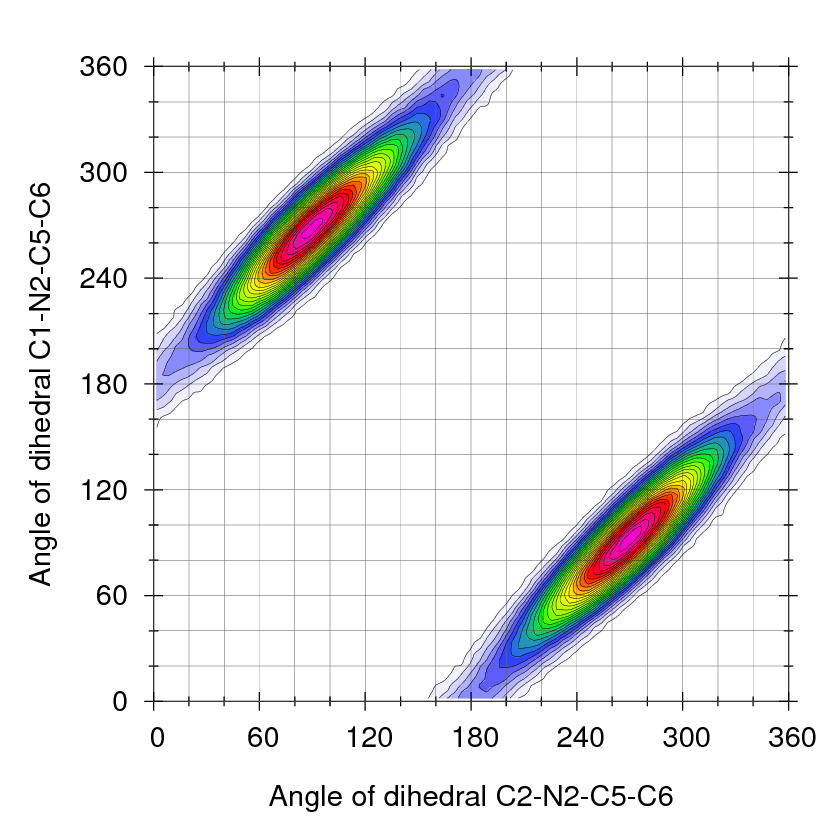
\includegraphics[width=.4\linewidth]{koller.png}}%
\subfloat[Batista~\textit{et al.}~\cite{Batista_2015}]{%  
  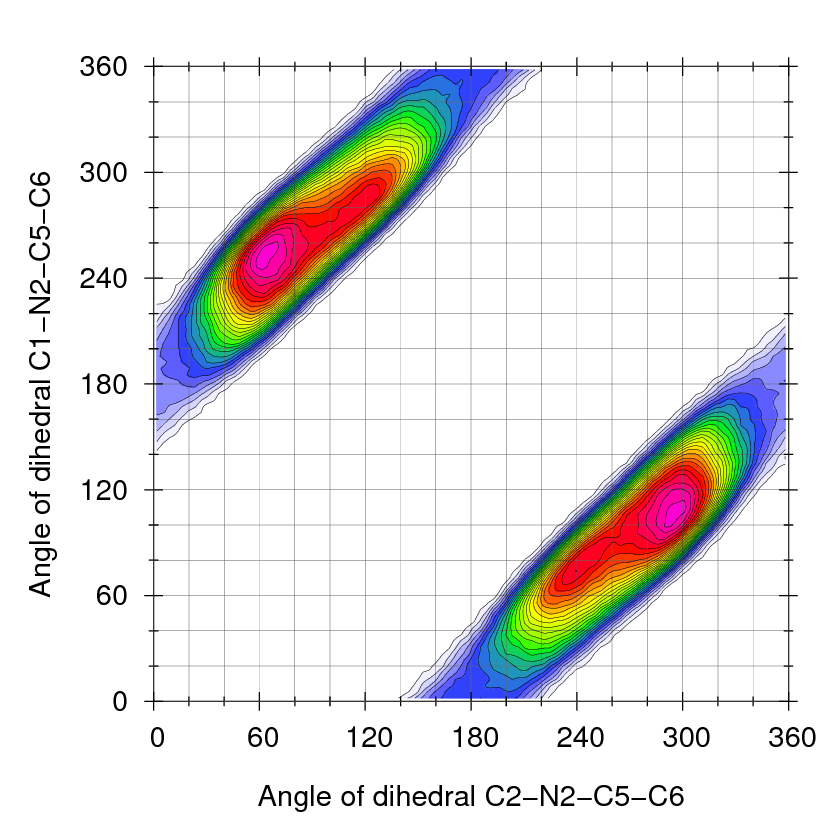
\includegraphics[width=.4\linewidth]{batista.png}}%
  
\subfloat[Liu~\textit{et al.}~\cite{Liu_2014}]{%
  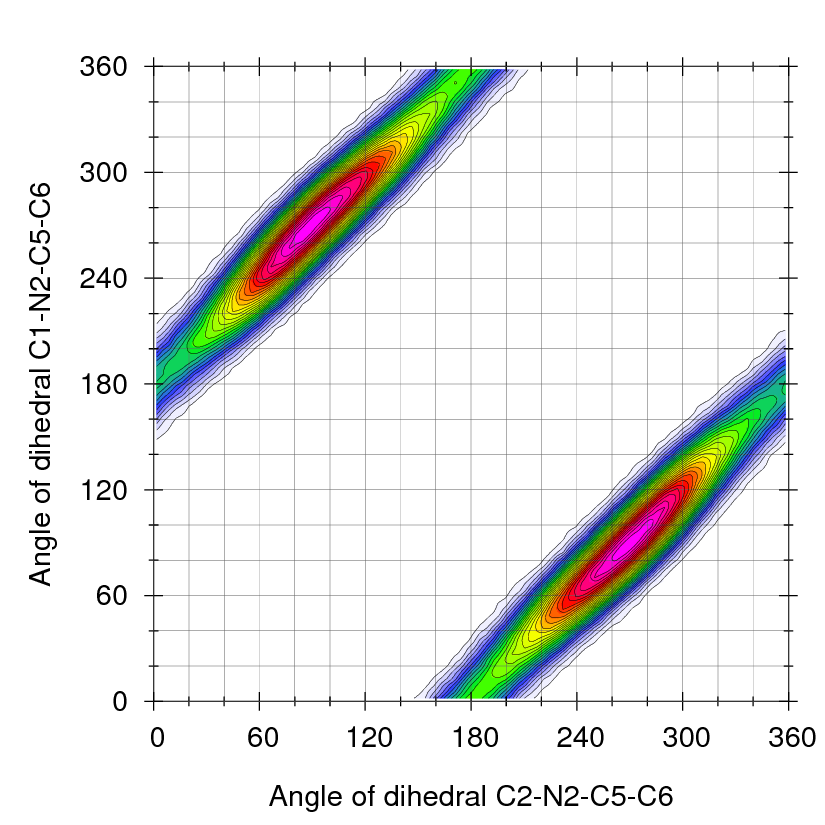
\includegraphics[width=.4\linewidth]{Liu.png}}%
\subfloat[Weber and Kirchner~\cite{Weber_2016}]{%
  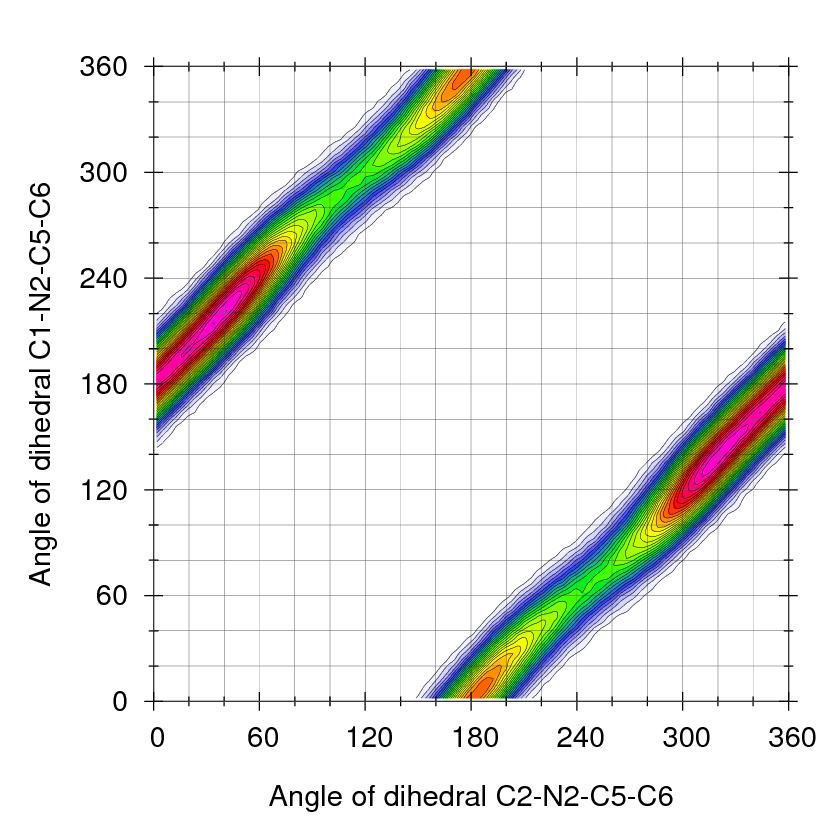
\includegraphics[width=.4\linewidth]{Weber.png}}%
\caption{Combined distribution function of the dihedral angles of C1-N2-C5-C6 and C2-N2-C5-C6, as sampled in NPT-MD simulations of 250 ion pairs for each model of \ce{[emim][B(CN)_4]}.}
\label{fig:dihedrals_emim}
\end{figure*}

A study of dihedrals was also carried out for \ce{[emim][NTf_2]}.
The CDF of the dihedrals angles of C1-N2-C5-C6 and C2-N2-C5-C6, shown in Fig.~\ref{fig:die_ntf2}(a), resembles the results of Fig.~\ref{fig:dihedrals_emim}(d), but the most likely angle of C1-N2-C5-C6 is 0$^{\circ}$.
This similarity was expected as both models of \ce{[emim]^+} are based on the force field developed by Canongia-Lopes and P\'{a}dua~ \cite{Canongia_Lopes_2006}.
With regards to the anion \ce{[NTf_2]^-}, Deetlefs \textit{et al.} \cite{Deetlefs_2006} have experimentally determined the conformer population of the liquid-phase and observed that \ce{[NTf_2]^-} is mostly in its \textit{trans} conformation.
Fig.~\ref{fig:die_ntf2}(b), which corresponds to the CDF for the contiguous C1-S1-N1-S2 and S1-N1-S2-C2 chains, qualitatively verifies the observation of Deetlefs \textit{et al.} \cite{Deetlefs_2006}.
Given the considerable flexibility of \ce{[NTf_2]^-}, a more rigorous strategy for building the rigid bodies is required.
Thus, the simulations of \ce{[emim][NTf_2]} were performed considering flexible ions and the DSF method, which results in a computed density of 1.495 $\pm$ 0.009 g/cm$^3$ with an error of 1.12\% with respect to the experimental value~\cite{Tokuda_2005}.

\begin{figure}[ht]
\centering
  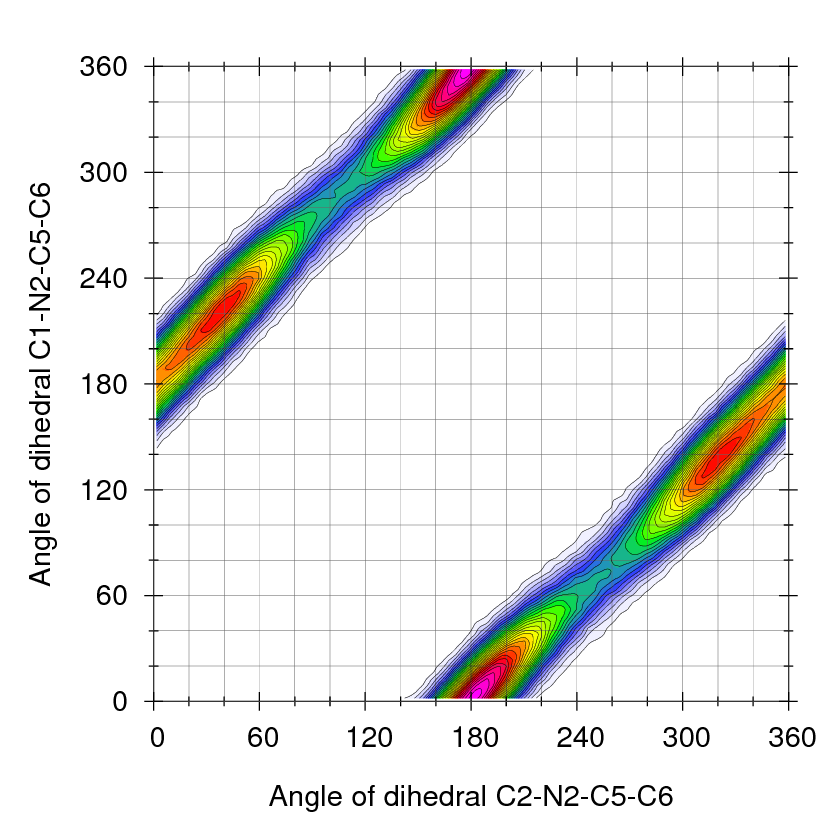
\includegraphics[width=\linewidth]{Ludwig.png}%

  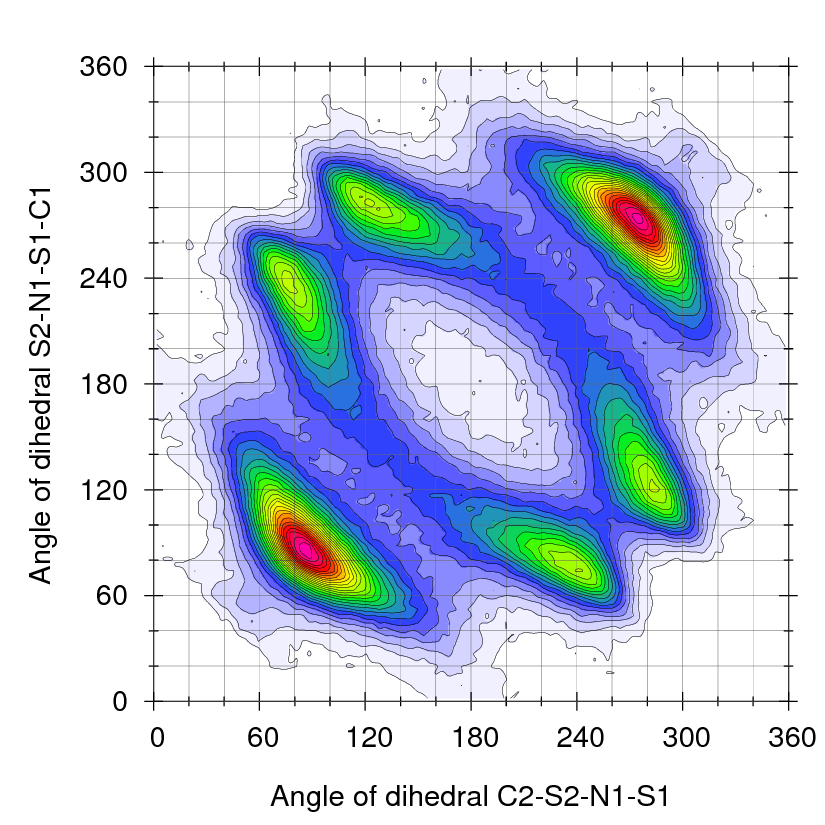
\includegraphics[width=\linewidth]{Ludwig_anion.png}%
\caption{Combined distribution function of (a) the dihedral angles of C1-N2-C5-C6 and C2-N2-C5-C6, and (b) of the dihedral angles of the contiguous  C1-S1-N1-S2 and S1-N1-S2-C2 chains, obtained from NPT-MD simulations of 250 molecules of \ce{[emim][NTf_2]}.}
\label{fig:die_ntf2}
\end{figure}

\begin{table*}
\begin{threeparttable}
\caption{Comparison of predicted and experimental densities for differents models of \ce{[emim][B(CN)_4]} via NPT-MD simulations at $T = 298.0~\text{K}$ and $P = 1.0~\text{atm}$. The experimental density is $\rho^{\text{exp}}$ = 1.036 g/cm$^{3}$~\cite{Doma_ska_2011}.}
\begin{tabular}{ c  c  c  c  c}  
\hline \hline
\ce{[emim][B(CN)_4]}&  $\rho_{\text{sim}}$ & error (\%)\tnote{a}  & $\rho_{\text{sim}}$ & error (\%)\tnote{a} \\
model & (g/cm$^{3}$) &  &  (g/cm$^{3}$) &  \\
			\hline
& \multicolumn{2}{c}{Flexible ions/Ewald method} & \multicolumn{2}{c}{Rigid ions/DSF method} \\
Koller y col. \cite{Koller_2012}    & 1.046 & 1.0 & 1.038 & 0.2 \\
Batista y col. \cite{Batista_2015}  & 0.989 & 4.6 & 0.988 & 4.7 \\
Liu y col. \cite{Liu_2014}          & 1.001 & 3.4 & 0.991 & 4.4 \\
Weber y Kirchner. \cite{Weber_2016} & 1.015 & 2.1 & 1.022 & 1.4  \\
 \hline \hline
\label{table:props_dsf} 
\end{tabular}
\begin{tablenotes}
\item[a] error = 100 $\times$($\rho^{\text{exp}}$$ - $$\rho^{\text{sim}}$)/$\rho^{\text{exp}}$.
\end{tablenotes}
\end{threeparttable}
\end{table*}

\subsection{Henry constant of \ce{CO_2} in \ce{[emim][B(CN)_4]} and \ce{[emim][NTf_2]}}
\label{sec:henry_results}

In Table \ref{table:henry} we present the results of the solvation free energies of \ce{CO_2} along with the Henry constants ($K_s$) obtained by means of Eq.~\eqref{eq:henry_eq}.
Table~\ref{table:henry} also contains the experimental $K_s$ reported by Mahurin \textit{et al.} \cite{Mahurin_2010} and Finotello \textit{et al.} \cite{Finotello_2008}.
The uncertainties in $K_s$ were calculated using standard error propagation.

\begin{table*}
\centering
\begin{adjustbox}{width=1\textwidth}
\begin{threeparttable}
\caption{Results of solvation free energies and Henry constants of \ce{CO_2} in \ce{[emim][B(CN)_4]} and \ce{[emim][NTf_2]} at $T$ = $298.15~\text{K}$ and $P$ = $1~\text{atm}$.
The experimental Henry constants in \ce{[emim][B(CN)_4]} and \ce{[emim][NTf_2]} correspond to 38.9 $\pm$ 0.03 atm~\cite{Mahurin_2010} and 39.0 $\pm$ 0.1 atm \cite{Finotello_2008}, respectively.}
\begin{tabular}{ c c c  c  c  c  c }  
\toprule
Model & $\tilde{\rho}_{\text{sim}}$ & $\Delta G_{\,\text{LJ}}$  & $\Delta G_{\,\text{Coul}}$  & $\Delta G_{\,\text{sim}}$ & $K_{s}$ & error (\%)\tnote{a}\\
& (mol/dm$^{3}$) & (kcal/mol) & (kcal/mol) &  (kcal/mol) & (atm)  &  \\
			\hline
			\multicolumn{4}{c}{\ce{[emim][B(CN)_4]}} & \multicolumn{2}{c}{\cellcolor{gray!25}$K_{s}^{\text{exp}}$ = 38.9 $\pm$ 0.03 atm~\cite{Mahurin_2010}}\\
			\hline
Koller \textit{et al.} \cite{Koller_2012} & 4.5925 & 0.45 $\pm$ 0.01 & -1.06 $\pm$ 0.02 & -0.61 $\pm$ 0.02 & 40 $\pm$ 1 & 2.8 \\
Batista \textit{et al.} \cite{Batista_2015} & 4.3700 & 0.378 $\pm$ 0.008 & -1.24 $\pm$ 0.01  & -0.86 $\pm$ 0.01 & 24.9 $\pm$ 0.5 & 38.9 \\
Liu \textit{et al.} \cite{Liu_2014} & 4.3815 & 0.226 $\pm$ 0.009 & -1.11 $\pm$ 0.01 & -0.88 $\pm$ 0.01 & 24.3 $\pm$ 0.5 & 37.6  \\
Weber y Kirchner \cite{Weber_2016} & 4.5221 & 0.478 $\pm$ 0.009 & -1.23 $\pm$ 0.02 & -0.75 $\pm$ 0.02 & 31 $\pm$ 1 & 20.3  \\
\hline
		\multicolumn{4}{c}{\ce{[emim][NTf_2]}} & \multicolumn{2}{c}{ \cellcolor{gray!25} $K_{s}^{\text{exp}}$ = 39.0 $\pm$ 0.1 atm~\cite{Finotello_2008}}\\
		\hline
 K\"{o}ddermann \textit{et al.} \cite{K_ddermann_2007} &3.8205 & 0.389 $\pm$ 0.005 & -0.901 $\pm$ 0.006& -0.512 $\pm$ 0.008 & 39.4 $\pm$ 0.5  & 0.97  \\
 \bottomrule
\label{table:henry} 
\end{tabular}
\begin{tablenotes}
\item[a] error = 100 $\times$ $\abs{(K_s^{\text{exp}} - K_s^{\text{sim}})/K_s^{\text{exp}}}$.
\end{tablenotes}
\end{threeparttable}
\end{adjustbox}
\end{table*}

It should be pointed out that the result of $\Delta G_{\text{sim}}$ obtained for the model of Liu \textit{et al.} \cite{Liu_2014} is statistically identical to the value reported by those authors \cite{Liu_2014_1}, who applied the BAR method \cite{Bennett_1976} to independent sampling of $\lambda_{\,\text{vdW}}$ and $\lambda_{\, \text{Coul}}$.
Moreover, the $\Delta G_{\text{sim}}$ in \ce{[emim][NTf_2]} is very close to the value obtained by Kerl \textit{et al.} \cite{Kerl__2017} ($-0.534$ kcal/mol, with no uncertainty reported) using the FEP method \cite{Zwanzig_1954}.
These consistencies have served for validating the methodological approaches of this work.

From Table \ref{table:henry} one can see that the model of Koller \textit{et al.} \cite{Koller_2012} best reproduces the experimental value of $K_s$.
If we look at the $\Delta G_{\lambda_{\,\text{vdW}}}$ profiles in Fig.~\ref{fig:deltag}, we observe that for the models of Batista \textit{et al.} \cite{Batista_2015} and Liu \textit{et al.}~\cite{Liu_2014} the maximum occurs at lower values of energy, suggesting that these models underestimate the interatomic interactions, which may also explain their failure to reproduce the experimental density.

\begin{figure}[ht]
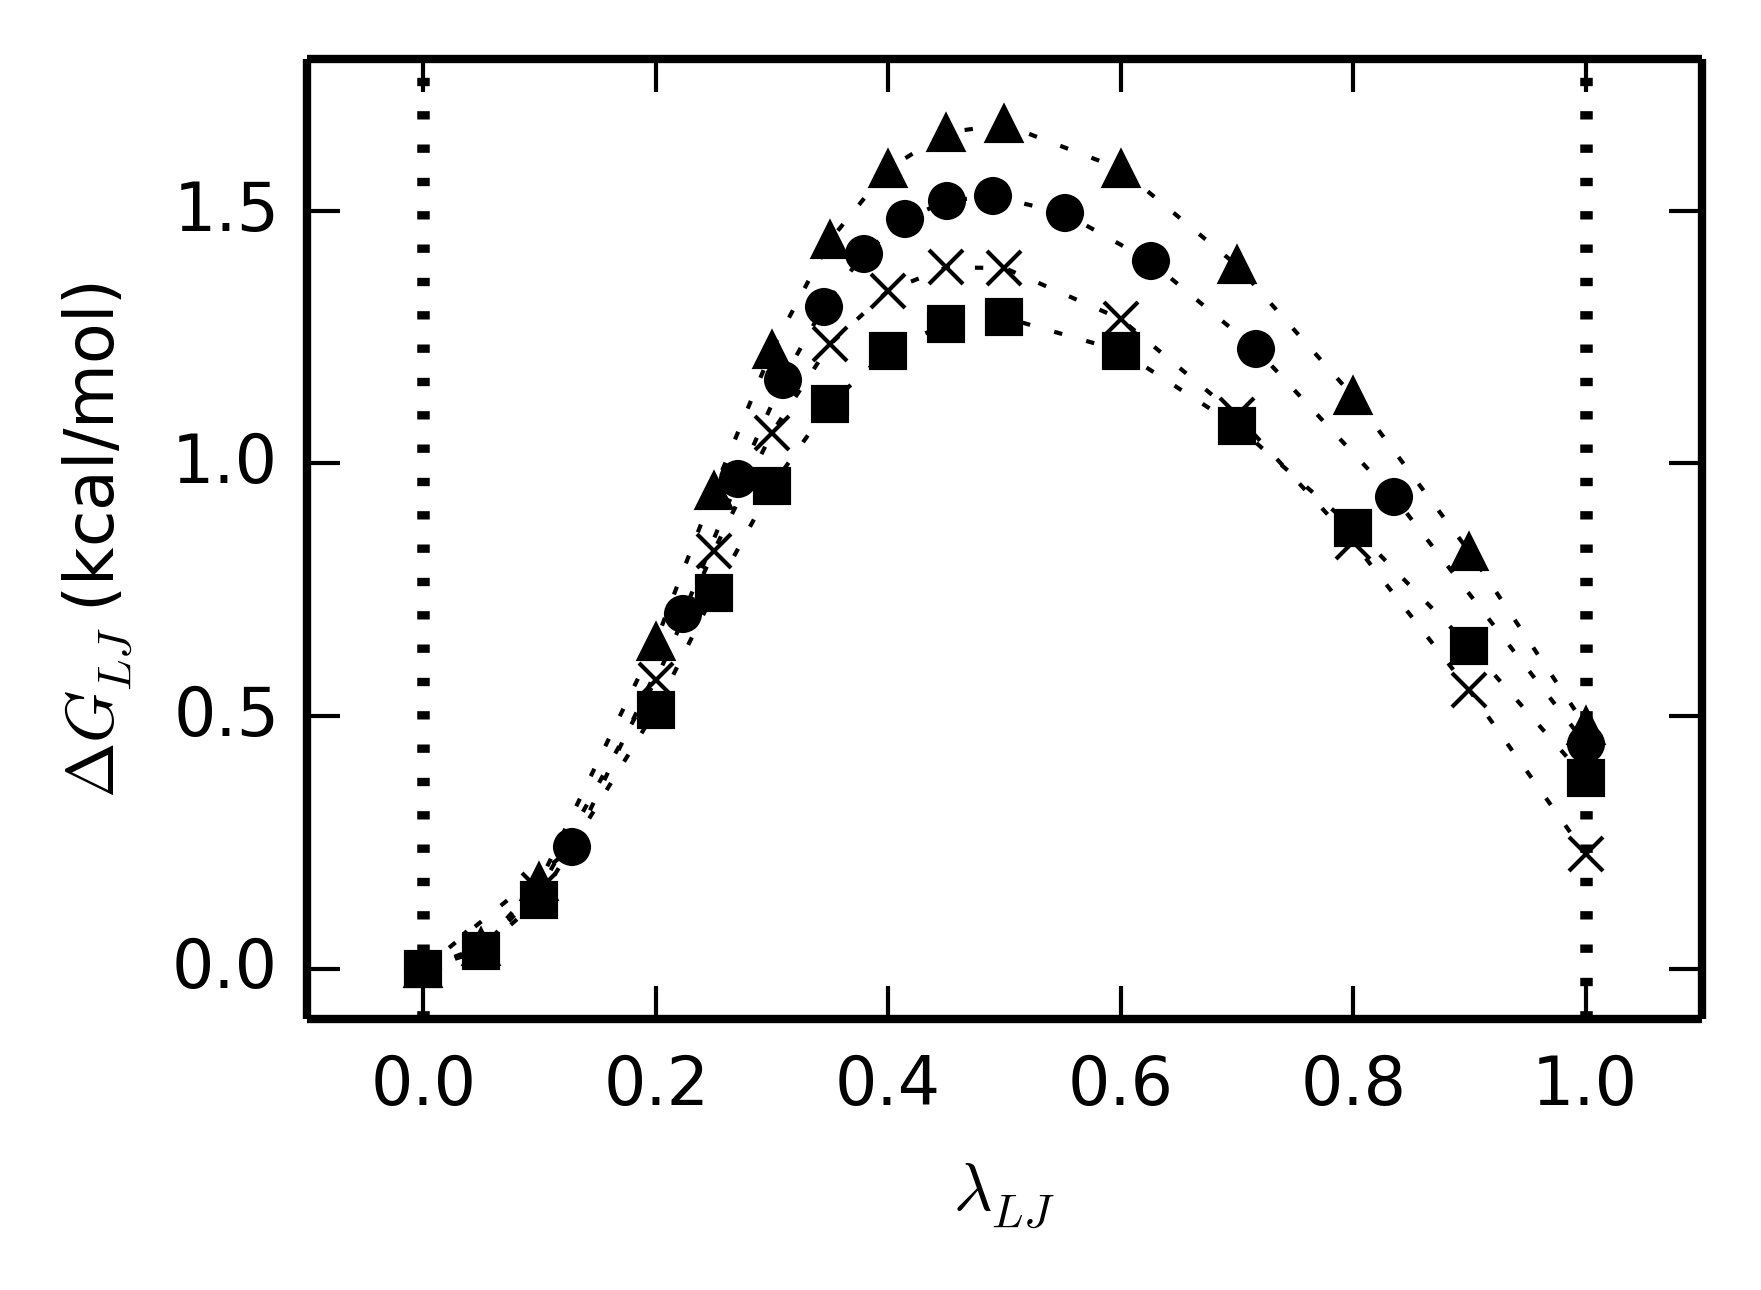
\includegraphics[width=\linewidth]{free_energy_paper}
\caption{$\Delta G_{\lambda_{\,\text{vdW}}}$ profiles corresponding to the insertion of a \ce{CO_2} molecule in \ce{[emim][B(CN)_4]}, which was modeled according to the force fields of (circles) Koller \textit{et al.} \cite{Koller_2012}, (squares) Batista \textit{et al.} \cite{Batista_2015}, (up triangles) Liu \textit{et al.} \cite{Liu_2014}, and (x) Weber y Kirchner \cite{Weber_2016}.}
\label{fig:deltag}
\end{figure}

The $\Delta G_{\, \text{sim}}$ values for the models of Koller \textit{et al.} \cite{Koller_2012} and K\"{o}ddermann \textit{et al.} \cite{K_ddermann_2007} suggest a more favorable solvation of \ce{CO_2} in \ce{[emim][B(CN)_4]} than in \ce{[emim][NTf_2]}. 
The spatial distribution functions (SDFs) \cite{Svishchev_1993} shown in Figs.~\ref{fig:sdf_ions} confirm this result.
The SDFs of the ions around a \ce{CO_2} molecule were obtained by using the software packages TRAVIS \cite{Brehm_2011} and VMD \cite{HUMP96}.
For that, we carried out NPT-MD simulations of \ce{CO_2}-\ce{[emim][B(CN)_4]} and \ce{CO_2}-\ce{[emim][NTf_2]} systems with a \ce{CO_2} molar fraction of 0.1.
The isovalues were visually determined so as to observe the first solvation shell.
If we compare Figs.~\ref{fig:sdf_ions} (a) and (b), one notes that the region with a low probability of finding an ion is larger for \ce{[emim][NTf_2]}.
Also, the first solvation shell due to [B(CN)\textsubscript{4}]$^{-}$ occurs at a slightly shorter distance than for \ce{[NTf_2]^-}, as one sees from Fig.~\ref{fig:sdf_ions} (c).
\begin{figure}[ht]
\centering
\subfloat[]{%
  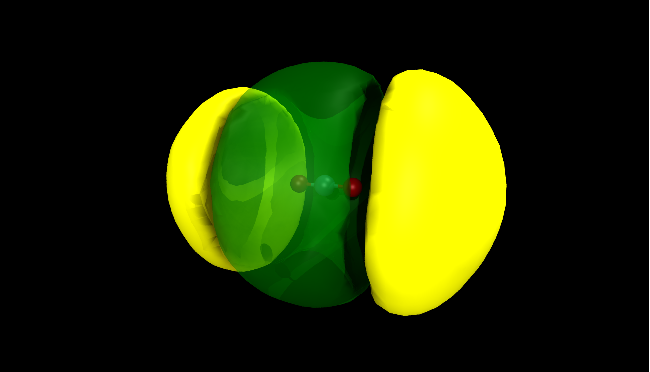
\includegraphics[width=\linewidth]{kollerall.pdf}%
}

\subfloat[]{%
  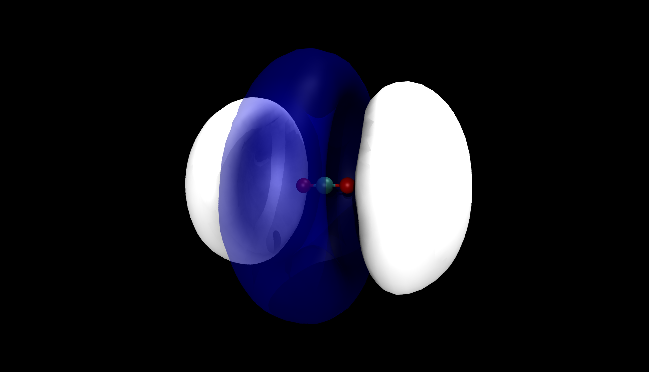
\includegraphics[width=\linewidth]{ludwigall.pdf}%
}

\subfloat[]{%
  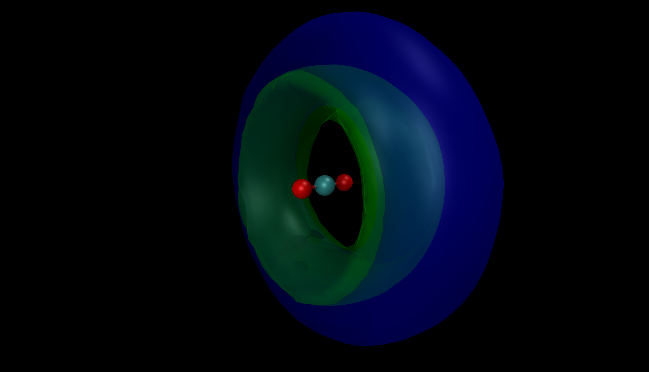
\includegraphics[width=\linewidth]{anionanion.pdf}%
}
\caption{Spatial distribution functions (SDFs) of (a) \ce{[B(CN)_4]^-} (green) and \ce{[emim]^+} (yellow) at the isosurface values of 0.138 and 0.12, respectively; and of (b) \ce{[NTf_2]^-} (blue) and \ce{[emim]^+} (white) at the isosurface values of 0.086 and 0.063, respectively.
Fig. (c) corresponds to the SDFs of the anions plotted together.}
\label{fig:sdf_ions}
\end{figure}

\subsection{Study of concentrated solutions of \ce{CO_2} in \ce{[emim][B(CN)_4]} and \ce{[emim][NTf_2]}}
\label{sec:results_conc}

Since concentrated solutions are the more likely scenario in \ce{CO_2} capture processes, we have also carried out simulations at the thermodynamic conditions specified in Table~\ref{table:solv}, which correspond to similar values of \ce{CO_2} molality.
Note that the differences in the \ce{CO_2} molar fractions clearly exemplifies the observation made by Carvalho \textit{et al.} \cite{Carvalho_2016}, mentioned at the introduction of this paper.

\begin{table*}
\centering
\begin{threeparttable}
\caption{Thermodynamic conditions employed in the solvation study at high concentrations of \ce{CO_2} in \ce{[emim][B(CN)_4]} and \ce{[emim][NTf_2]}~\cite{Makino_2014,Schilderman_2007}.}
\begin{tabular}{ c  c  c  c  c  }  
\toprule
Ionic liquid & T (K)  & P (atm)  & molar fraction $x_s$ & molality $m_s$ \\
\midrule		
\ce{[emim][B(CN)_4]}~\cite{Koller_2012} & 313.15 & 21 & 0.352 & 2.4  \\
\ce{[emim][NTf_2]}~\cite{K_ddermann_2007}  & 312.13 & 37 & 0.479 & 2.35  \\
 \bottomrule
\label{table:solv} 
\end{tabular}
\end{threeparttable}
\end{table*}

For each system, in Fig.~\ref{fig:pressure} we show our predictions of the gas-phase pressure ($P_s$), as described in Sec.~\ref{sec:partial_pressure}.
The dotted lines are the experimental pressures, which correspond to the specified values ($P$) in the liquid-phase simulation.
Note that our results reproduce what is experimentally observed, in the sense that the calculated $P_s$ is considerably lower for \ce{CO_2}-\ce{[emim][B(CN)_4]}.
In addition, we see that in this case the correction to the ideal gas assumption is almost negligible, as $P_s$ is very close to the fugacity ($f^g_s$).
The solvation free energies obtained for \ce{CO_2}-\ce{[emim][B(CN)_4]} and \ce{CO_2}-\ce{[emim][NTf_2]} were -0.755 $\pm$ 0.01 kcal/mol and -0.542 $\pm$ 0.005, respectively.
However, since we simulated a different number of \ce{CO_2}, we cannot draw any definite conclusion regarding the presence of stronger interactions with \ce{[emim][B(CN)_4]}, which could explain the higher solubility.

\begin{figure}[ht]
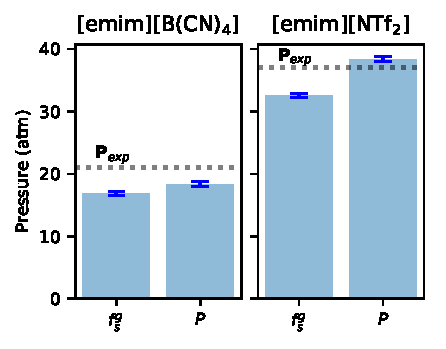
\includegraphics[width=\linewidth]{pressure_est.pdf}
\caption{Prediction of the gas-phase fugacity and partial pressure of \ce{CO_2} for the systems \ce{CO_2}-\ce{[emim][B(CN)_4]} and \ce{[emim][NTf_2]}.}
\label{fig:pressure}
\end{figure}

\subsection{Inifinite-dilution activity coefficient in \ce{[emim][B(CN)_4]}}
\label{sec:act_results}

Having selected the model of \ce{[emim][B(CN)_4]} that best reproduces the experimental $K_s$ of \ce{CO_2}, we next calculate the infinite-dilution activity coefficients ($\gamma^{\, \infty}$) of benzene, hexane, cyclohexane, ethanol and water in \ce{[emim][B(CN)_4]}.

The task of accurately predicting $\gamma^{\, \infty}$ is challenging since, according to Eq.~\eqref{eq:gamma_inf}, one should reproduce the solvation free energies in both the pure solute and the solvent.
In Table~\ref{table:mu_solutes} we show the simulated densities and the solvation free energies $(\Delta G^{0}_{\text{sim}})$ of the pure solutes, which we compare against the experimental data extracted from the work of Chang~\cite{Chang_2009}.
It should be pointed out that we were unable to find the experimental $\Delta G^{0}_\text{exp}$ for cyclohexane.
Note that only in the case of ethanol we successfully predicted the $\Delta G^{0}_\text{exp}$.
The relative errors for the other solutes are around 10\%.

The results of $\gamma^{\, \infty}$ are presented in Table~\ref{table:gamma}.
For benzene and water, the predictions are very accurate, but this may be due to fortuitous error compensations given the divergences shown in Table~\ref{table:mu_solutes}.
From Table \ref{table:gamma}, one sees that the experimental $\gamma^{\, \infty}$ for hexane at $298.15~\text{K}$ and $303~\text{K}$ considerably differ.
It is therefore difficult to assess the reliability of our results in this case.

\begin{table*}
\centering
\begin{adjustbox}{width=1\textwidth}
\begin{threeparttable}
\caption{Solvation free energy at $T = 298.15~\text{K}$ for the pure solutes benzene, hexane, cyclohexane, ethanol and water.}
\begin{tabular}{ c c c c c c c c }
\toprule
Solute & $\rho_{\text{sim}}$ & error (\%)\tnote{a} & $\Delta G_{\,\text{LJ}}$  & $\Delta G_{\,\text{Coul}}$  & $\Delta G^{0}_{\,\text{sim}}$ & $\Delta G^{\text{0,exp}}$   & error (\%)\tnote{a}\\
 & (g/cm$^{3}$) &  & (kcal/mol) &  (kcal/mol) &  (kcal/mol)   &  \\
\hline
benzene OPLS-AA   & 0.8611 $\pm$ 0.0002 & 1.4 & -3.75  $\pm$ 0.02 & -0.381 $\pm$ 0.007 & -4.14 $\pm$ 0.02 & -4.56 & 9.32  \\
hexane OPLS-AA    & 0.6513 $\pm$ 0.0003 & 0.5 & -3.67  $\pm$  0.03 & 0.011 $\pm$ 0 & -3.66 $\pm$ 0.03 & -4.06 & 9.90 \\
cyclohexane & 0.7692 $\pm$ 0.0007 & 0.6 & -4.39 $\pm$ 0.01 & 0 & -4.39 $\pm$ 0.01 & - & -  \\
ethanol TRAPPE-UA   & 0.781 $\pm$ 0.008 & 1.01  &-0.93 $\pm$ 0.01 & -4.15 $\pm$ 0.02  & -5.08  $\pm$ 0.02  & -5.08 & 0 \\
water TIP4P/2005   &  0.9948 $\pm$ 0.0003 & 0.2 & 2.015 $\pm$ 0.004 & -9.01 $\pm$ 0.02 & -6.99 $\pm$ 0.02 & -6.33  &10.43 \\
 \bottomrule
\label{table:mu_solutes} 
\end{tabular}
\begin{tablenotes}
\item[a] error = 100 $\times$ $\abs{(Z^{\text{exp}} - Z^{\text{sim}})/Z^{\text{exp}}}$.
\end{tablenotes}
\end{threeparttable}
\end{adjustbox}
\end{table*}

\begin{table*}
\centering
\begin{adjustbox}{width=1\textwidth}
\begin{threeparttable}
\caption{Infinite-dilution activity coefficients in \ce{[emim][B(CN)_4]} at $T = 298.15~\text{K}$ of the pure solutes benzene, hexane, cyclohexane, ethanol, and water.}
\begin{tabular}{c c c c c c  >{\columncolor[gray]{0.8}} c}  
\toprule
Solute & $\Delta G_{\,\text{LJ}}$  & $\Delta G_{\,\text{Coul}}$  & $\Delta G_{\,\text{sim}}$  & $\gamma^{\,\infty,\text{sim}}$ & $\gamma^{\, \infty,\text{exp}}$ & $\gamma^{\, \infty,\text{exp}}$  \\
 & (kcal/mol) & (kcal/mol) &  (kcal/mol)  &  & (298.15 K) \cite{Doma_ska_2011} & (303 K) \cite{Yan_2010} \\
\midrule % inserts single-line
hexane OPLS-AA & -2.13 $\pm$ 0.04 & -0.152 $\pm$ 0.007 & -2.282 $\pm$ 0.04 & 6.2 $\pm$ 0.5 & 33.8 & 20.97  \\
cyclohexane& -2.75 $\pm$ 0.06 & - & -2.75 $\pm$ 0.06 & 9 $\pm$ 1 & 16.7 & 13.82 \\
benzene OPLS-AA  & -2.23 $\pm$ 0.05 & -1.29 $\pm$ 0.04 & -3.52 $\pm$ 0.06 & 1.2 $\pm$ 0.1 & 1.13 & 1.31 \\ 
ethanol TRAPPE-UA& -0.73 $\pm$ 0.02 & -4.10 $\pm$ 0.04 & -4.83 $\pm$ 0.04 & 0.41 $\pm$ 0.03 & 1.58 & 1.64  \\
water TIP4P/2005& 1.38 $\pm$ 0.008 & -6.32 $\pm$ 0.03 & -4.94 $\pm$ 0.03 & 2 $\pm$ 1 & 2.65 & 2.24 \\
 \bottomrule
\label{table:gamma} 
\end{tabular}
\end{threeparttable}
\end{adjustbox}
\end{table*}
\section{Concluding remarks}
\label{sec:conclusion}

One of the goals of this paper was to compare various available models of \ce{[emim][B(CN)_4]} in terms of their capability to reproduce the experimental Henry constant of \ce{CO_2}.
We have found that only the force field developed by Koller \textit{et al.} \cite{Koller_2012} is able to perform such task, with a small relative error of 2.8 \%.
A key factor for its success seems to be the reparametrization of the LJ parameters for the boron atom carried out in that work, which also allows to accurately reproduce the experimental density of the pure substance.

We focused also on exploring alternative simulation strategies with the goal of gaining computational efficiency.
Particularly, for both \ce{[emim][B(CN)_4]} and \ce{[emim][NTf_2]}, we concluded that the DSF method with $\alpha$ = 0.2 {\AA}$^{-1}$ is a suitable strategy.
Other improvement was the use of rigid bodies to simulate \ce{[emim][B(CN)_4]}.
This required preliminary simulations in order to examine the flexibility of the ethyl chain in \ce{[emim]^+} and the analysis was greatly facilitated by employing useful visualization tools.
Besides the properties already mentioned, the different models showed quite different behaviors, as well.
This lack of consistency is one of the reasons why in industry molecular simulation has not become a routinely tool yet.

The solvation free energy results at infinite-dilution condition suggest a slightly more favorable solvation of \ce{CO_2} in \ce{[emim][B(CN)_4]} than in  \ce{[emim][NTf_2]}.
However, this picture changes at high concentrations: the simulations correctly predicted a considerable lower pressure to dissolve a certain mass of \ce{CO_2} in \ce{[emim][B(CN)_4]}.

Finally, we employed the model of Koller \textit{et al.} \cite{Koller_2012} to predict infinite-dilution activity coefficients of various solutes.
In this case, the results were not satisfactory given the large errors in the free energy calculations of the pure solutes, making necessary a revision of their force fields in a future work.

\section*{Acknowledgments}
The authors acknowledge the financial support provided by Petrobras (project code CENPES 16113). 

\section*{References}

\bibliography{mybibfile}

\end{document}


